%% ch1.tex
\chapter{Neurophysiology Background}
\label{ch:neurobackgnd} 
%%%%%%%%%%%%%%%%%%%%%%%%%%%%%%%%%%%%%%%%%%%%%%%%

% 1111111111111111111111111111111111111111111111111111111111111111111111111111

\section{Structure of the Brain}
\label{sec:struct}

The brain together with the spinal cord make up the central nervous system, the body's sensory analysis and decision making system. \cite{Kandel_2002_PrinciplesNeuralSc,Sherwood_2001_cell2sys,Nunez_2006_ElecFieldsBrain} provide the following information regarding the anatomy of the brain. The brain can be subdivided into two main regions, the brainstem and cerebrum. The cerebrum is structurally divided into two main regions each called a cerebral hemisphere.  The outer layer of the hemispheres is known as the cerebral cortex. The cortex is a much folded structure which is estimated to contain in the order of $10^{10}$ nerve cells or $\it{neurons}$ \cite[Ch. 1]{Nunez_2006_ElecFieldsBrain}.  The cortex contains both ``grey matter'' and ``white matter''.  Grey matter is a layer containing a high density of neuron cell bodies while, the white matter, located underneath the grey matter, is largely composed of  nerve  fibers or $\it{axons}$.  The cortex is further divided into four main lobes, each with its own function specification, see Figure~\ref{fig:brainsurf}.  The brain stem connects the spinal cord to the cerebral cortex, via the thalamus, a deep brain structure which gates the information flow from the brainstem to the cortex, see Figure~\ref{fig:brainmid}.\\

\begin{figure} [hbt]
\centering
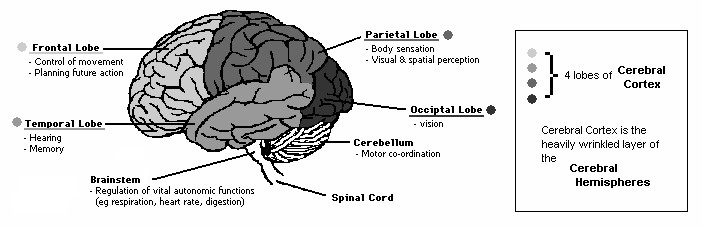
\includegraphics[height=2.1in]{figures/070108_brain_parts}
\caption{Surface view of the brain, illustrating the main lobes of the cerebral cortex and their basic functions, taken in part from \cite{corteximage} }
\label{fig:brainsurf}
\end{figure}

\section{Epilepsy}
\label{sec:epilepsy}

The International League Against Epilepsy (ILAE) defines an epileptic event as ``a transient occurrence of signs and symptoms due to abnormally excessive or synchronous neuronal activity in the brain''\cite{Fisher_2005_DefinitionsfromILAE}.  Epilepsy is defined as ``a disorder of the brain characterised by an enduring predisposition to generate epileptic seizures''\cite{Fisher_2005_DefinitionsfromILAE}, and is usually not diagnosed until more than one epileptic event has occurred.\\     



\section{Electroencephalography}
\label{sec:eeg}

Electroencephalography (EEG) is a record of the temporal fluctuations of electrical potentials recorded from electrodes on the human brain. \\


\subsection{Interpretation of the EEG}

subsection text.....